% !TeX spellcheck = en_US
\documentclass[french]{yLectureNote}

\title{Optique ondulatoire}
\subtitle{Physique}
\author{Paulhenry Saux}
\date{\today}
\yLanguage{Français}

\professor{F.Pettinari}
\usepackage{graphicx}%----pour mettre des images
\usepackage[utf8]{inputenc}%---encodage
\usepackage{geometry}%---pour modifier les tailles et mettre a4paper
%\usepackage{awesomebox}%---pour les boites d'exercices, de pbq et de croquis ---d\'esactiv\'e pour les TP de PC
\usepackage{tikz}%---pour deiffner + d\'ependance de chemfig
% \usepackage{tabularx}%---pour dimensionner automatiquement les tableaux avec variable X
\usepackage{awesomebox}%---Pour les boites info, danger et autres
\usepackage{menukeys}%---Pour deiffner les touches de Calculatrice
\usepackage{fancyhdr}%---pour les en-t\^ete personnalis\'ees
\usepackage{blindtext}%---pour les liens
\usepackage{hyperref}%---pour les liens (\`a mettre en dernier)
\usepackage{caption}%---pour la francisation de la l\'egende table vers Tableau
\usepackage{pifont}
\usepackage{array}%---pour les tableaux
\usepackage{lipsum}
\usepackage{yFlatTable}
\usepackage{multicol}
\newcommand{\Lim}[1]{\lim\limits_{\substack{#1}}\:}
\renewcommand{\vec}{\overrightarrow}
\newcommand{\N}[0]{\mathbb{N}}
\newcommand{\dd}{\mathrm{d}}
\newcommand{\norm}[1]{||\vec{#1}||}
\newcommand{\fo}{\psi(\vec{r},t)}
\newcommand{\foe}{\psi(\vec{r},t)\*}
\newcommand{\HH}{\hat{H}}
\newcommand{\hb}{\hbar}
\newcommand{\lap}{\nabla^2}
\newcommand{\lapcc}{\frac{\partial^2 }{\partial x^2}+\frac{\partial^2 }{\partial y^2}+\frac{\partial^2 }{\partial z^2}}
\newcommand{\mpsi}{\(\psi\)}
\newcommand{\und}{\underline}
\newcommand{\dph}{\Delta\varphi}
\begin{document}
\setcounter{chapter}{1}
\chapter{Interférences d'ondes lumineuses}

% \section{Principe de superposition}
% L'équation d'onde est linéaire. Cela siginfie que les solutions forment un espace vectoriel. Cela nous permetd d'additionner les fonctions d'onde entre elles.

Si 2 sources éclairent un point, on a une fonction d'onde totale \(\und{\fo_1} + \und{\fo_2}\). Cependant, on ne peut pas le faire avec l'intensité car elle dépend du carré des fonctions\marginTips{En général, si \(\fo = \fo_1+\fo_2\), on a pas toujours \(I = I_1+I_2\).}.

% On dit que 2 ondes inteférent si \(I \neq I_1+I_2\). Si \(I>I_1+I_2\), on parle d'interférences constrctives, dans le cas contraire, ce sont des interfére,cesd esctrcutives.

\section{Role de la pulsation dans les interférences}
La superposition de \(\psi = \fo_1+\fo_2\) des deux ondes a pour intensité  \(I = 2<(\psi_1+\psi_2)^2> = |\und{\fo_1}+\und{\fo_2}|^2 = I_1+I_2 + 2Re(\und{\fo_1}\und{\foe_2})\)

La partie réelle est le terme d'interférence. Si les 2 fonctions d'onde de pulsation \(\omega_1\) et \(\omega_2\), alors en un point M, on a
\begin{flalign*}
\und{\fo_1} &= \und{\varphi_{1,0}} e^{-w\omega_1t}\\
\und{\fo_2} &= \und{\varphi_{2,0}} e^{-w\omega_2t}\\
\end{flalign*}
On a alors \(I_1 = |\und{\varphi_{1,0}}|^2\) et \(I_2 = |\und{\varphi_{2,0}}|^2\) et \(2Re(\und{\fo_1\foe_2}) = 2AB \cos((\omega_2-\omega_1)t + (\varphi_2-\varphi_1))\)

On remarque que le terme d'interférence oscille à la pulsation \(\omega_2-\omega_1\).
% très rapidement si \(\omega_1\neq \omega_1\) dans le visible. Comme on ne voit qu'une moyenne, il sera impossible de mesurer l'interféence car les oscillations sont trop rapides.

% En revanche, si \(\omega_1=\omega_2\), le terme d'interférence est constant et donc observable.

On considère donc deux cas :
\begin{itemize}
 \item Si les 2 ondes ont la m\^eme pulsation (les ondes sont alors isochrones ou cohérentes)\marginTips{On parle de cohérence quand on peut définir la phase d'un objet par rapport à l'autre} : on somme les \(\fo\)
 \item Si les les pulsations sont différentes, on somme les \(I\)
\end{itemize}

\warningInfo{Battement}{Si les 2 pulsations sont très proches, le terme d'interférence dépend du temps, on parle alors de battement.}
\section{Interférence d'ondes isochrones}
\subsection{En un point}
On a 2 ondes \(\und{\fo_1}, \und{\fo_2}\) pouvant s'écrire comme \[\und{\psi_1(M)} = \und{\psi_{10}}(M)e^{-i(\omega t+\varphi(M))}\] et \[\und{\psi_2(M)} = \und{\psi_{20}}(M)e^{-i(\omega t+\varphi(M))}\] ou encore \(\psi_{10}e^{-i(\omega t + \varphi_1)}\) et \(\psi_{20}e^{-i(\omega t + \varphi_2)}\).

Les intensités devienent alors \(I_1(M) = |\und{\psi_1}| = \psi_{10}^2\) et \(I_2(M) = |\und{\psi_2}| = \psi_{20}^2\)

Par le principe de superposition, on a
% \(\und{\psi} = \und{\psi_1}+\und{\psi_2} = (\psi_{10}e^{-i\varphi_1}+ \psi_{20}e^{-i\varphi_2})e^{-i\omega t}\) et li'intebsité sera \(|\und{\psi}|^2 = |\psi_{10}e^{-i\varphi_1}+\psi_{20}e^{-i\varphi_2}| = (\psi_{10}e^{-i}+\psi_{20}e^{-i})(\psi_{10}e^{+i}+\psi_{20}e^{+i}) = \psi_{10}^2 + \psi_{20}^2 + \psi_{10}\psi_{20}(e^{-i(\varphi_1-\varphi_2)}+e^{+i(\varphi_1-\varphi_2)})\)
\explanation{c1}{le module carré d'un nombre complexe z est égal au produit de z par son conjugué complexe z∗ : \(|z|^2  =z\cdot z^*\)}
\explanation{c2}{On utilise l'identité d'Euler :  Dans ce cas, \(\theta=\varphi_1​−\varphi_2\)​. On remplace la somme des exponentielles par \(2\cos(\varphi_2-\varphi_1)\).}
\begin{flalign*}
|\und{\psi}|^2 &= |\psi_{10}e^{-i\varphi_1}+\psi_{20}e^{-i\varphi_2}|^2\explain{c1}{right}{0}{0.5}{×}\\
&= (\psi_{10}e^{-i}+\psi_{20}e^{-i})(\psi_{10}e^{+i}+\psi_{20}e^{+i}) \\
&= \psi_{10}^2 + \psi_{20}^2 + \psi_{10}\psi_{20}(e^{-i(\varphi_1-\varphi_2)}+e^{+i(\varphi_1-\varphi_2)})\\
&= I_1+I_2+2\sqrt{I_2I_2}\cos(\varphi_2-\varphi_1)\explain{c2}{right}{0}{0.5}{×}
\end{flalign*}
On remarque que le terme d'interférence dépend surtout de \(\varphi_1-\varphi_2 = \Delta \varphi\) qui est le déphasage des 2 ondes au point M.

Les interférences sont
\begin{itemize}
 \item constructives si \(\cos(\Delta \varphi)>0 \Rightarrow I>I_1+I_2\)
  \item destructives si \(\cos(\Delta \varphi)<0 \Rightarrow I<I_1+I_2\)
\end{itemize}
\subsubsection{M\^eme intensité}
Si les ondes ont la m\^eme intensité, l'expression devient\marginTips{Car \(\cos^2(\theta) = \frac12(1+\cos(2\theta))\)} \[I = 2I_0(1+\cos(\Delta \varphi)) = 4I_0\cos^2(\frac{\Delta \varphi}{2})\]
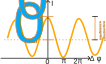
\includegraphics[scale=0.5]{interference}

Il est max (\(4I_0\)) si \(\Delta \varphi\) est un multiple de \(2\pi\). Les 2 ondes sont alors en phase. Dans le cas contraire, il est minimum (0) si \(\Delta \varphi = \pi+2\pi n\) et les 2 ondes sont en opposition de phase.

\begin{definition}[Ordre d'interférence]
C'est \[p = \frac{\Delta \varphi}{2\pi}\]
\end{definition}
L'internsité sera alors maximale si p est entier et minimale dans le cas contraire.
\subsubsection{Cas général}
Dans ce cas, \(I_1\neq I_2\) et \(I = I_1+I_2+2\sqrt{I_1I_2}\cos(\Delta \varphi)\). On obtient que
\begin{itemize}
 \item L'intensité maximale vaut alors \(I_1+I_2+2\sqrt{I_1I_2} = (\sqrt{I_1}+\sqrt{I_2})^2\)
 \item L'intensité minimale vaut alors \((\sqrt{I_1+\sqrt{I_2}})^2\)
\end{itemize}
On introduit la visibilité.
\begin{definition}[Visibilité]
\[V = \frac{I_{max-I_{min}}}{I_{max}+I_{min}}\leq 1\]
\end{definition}
Par exemple, si \(I_2=0.2I_1, V=0.75\)\marginInfo{Les interférences restent visibles m\^eme si il y a 2 odg de différence d'intensité entre les 2 ondes}.
\subsubsection{Interférogramme}
\begin{definition}[Interférogramme]
C'est la répartition spatiale de l'intensité résultant des interférences : \(I(\vec{r}) = I_1(\vec{r})+I_2(\vec{r})+2\sqrt{I_1I_2})\)
\end{definition}
En pratique, \(I_1(\vec{r})\) et \(I_2(\vec{r})\) varient peu mais pas \(\dph(\vec{r})\), qui peut varier beaucoup.
\checkInfo{Exemple}{Sur un écran, on peut avoir \(\dph(\vec{r}) = 2\pi n\) pour différentes points. On observe des zones brillantes pour \(\dph = 2\pi n\) et sombres pour \(\dph = \pi+2\pi n\). Il faut donc voir les interférences comme une redistribution spatiale de l'intensité.
}
\includegraphics[scale=0.5]{rect1}
\subsection{Intéfrérence de 2 ondes planes}
On prend \[\und{\fo_1} = \psi_{10}e^{i(\vec{k}\cdot \vec{r}-\omega t+\varphi_1)}\] et \[\und{\fo_2} = \psi_{20}e^{i(\vec{k}\cdot \vec{r}-\omega t+\varphi_2)}\] de m\^eme pulsation,  norme de vecteur d'onde mais \(\vec{k_1}\neq \vec{k_2}\)\marginInfo{Cependant, \(\norm{k_1} = \frac{n\omega}{c} = \norm{k_2}\). Seule la direction change.}.

On a
\explanation{c21}{Le second terme est un décalage uniforme que l'on peut choisir nul}
\explanation{c22}{\(\vec{k}\) est la différence entre les 2 vecteurs d'onde, il vaut ici \(2k\sin(\theta)\vec{e_z}\)}
\begin{flalign*}
\dph &= \phi_2-\phi_1\\
&= (\vec{k_2}\cdot \vec{r}+\varphi_2)- (\vec{k_1}\cdot \vec{r}+\varphi_1)\\
&= (\vec{k_2}- \vec{k_1})\cdot \vec{r}+(\varphi_2-\varphi_1)\explain{c21}{right}{0}{0.5}{}\\
&= \vec{k}\explain{c22}{right}{0}{0.5}{}
\end{flalign*}
On a \(I(\vec{r}) = I_1+I_2+2\sqrt{I_1I_2}\cos(2k\sin(\theta)z)\). On verra donc sur un écran des franges (lignes)\marginWarning{Pour avoir cette distance visible à l'œil nu (i = 1mm) et \(\lambda = 500 nm\), il faut \(\sin(\theta) = 2.5\cdot10^{-5}\). Il faut donc un très petit angle.}

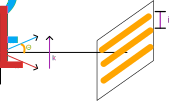
\includegraphics[scale=0.5]{schema3}
\begin{definition}[Interfrange]
C'est la distanxe entre les franges, notée \(i\) avec \[i = \frac{2\pi}{2k\sin(\theta)} = \frac{\lambda}{2\sin(\theta)}\]
\end{definition}
\subsection{Interférence entre de 2 ondes sphériques}
\subsubsection{Dispositif}
\includegraphics[scale=0.5]{dispo}

% On a \[\und{\fo_1} = \frac{A_1}{S_1M}e^{i(kS_1M-\omega t)}\] et \[\und{\fo_2} = \frac{A_1}{S_2M}e^{i(kS_2M-\omega t)}\] donc \(I_1(M) = |\frac{A_1}{S_1M}|^2\) et \(I_2(M) = |\frac{A_1}{S_2M}|^2\). On en déduit le déphasage\marginCheck{On utilise la relation de dispersion et on entroduit \(\delta\) al différence de marche.}
%
% \[\dph = k(S_2M-S_1M) = \frac{2\pi n}{\lambda_0}(S_2M-S_1M) = \frac{2\pi n}{\lambda_0}\delta \]
\subsubsection{Écran parallèle à l'axe des sources}
\includegraphics[scale=0.4]{ecran}

En supposant \(a<< D\) et en  introduisant ici la différence de marche \(\delta\) de 2 ondes on trouve \[\dph = \frac{2\pi}{\lambda_0}\delta\]

%TODO Fin CM eval---------------------------------
On note \(\fo_1 = \frac{A}{r_1}e^{i(kr_1-\omega t-\varphi_1)}\) et  \(\fo_2 = \frac{A}{r_2}e^{i(kr_2-\omega t-\varphi_2)}\)

L'intensité en M vaut \(I_1 = |\frac{A}{r_1}|^2, I_2 = |\frac{A}{r_2}|^2\) et la différence de phase
\newpage
\explanation{e1}{On suppose que \(\varphi_2-\varphi_1 = 0\).}

\begin{flalign*}
\Delta \varphi &= (kS_2M-\varphi_2) - (kS_1M-\varphi_1)\\
&= k(S_2M-S_1M)-(\varphi_2-\varphi_1)\\
&= \frac{2\pi}{\lambda_0}n(S_2M-S_1M)\explain{e1}{right}{0}{0.5}{×}\\
&=\frac{2\pi}{\lambda_0}((S_2M)-(S_1M))\\
&=\frac{2\pi}{\lambda_0}(\delta)
\end{flalign*}

On suppose que l'écran est loin des sources\marginInfo{Cela signifie que \(D>>a\) et M est proche du centre de l'écran, donc \(D>>x,y\)}

Sous ces hypothèses, on peut prendre \(I_1\simeq I_2 \simeq |\frac{A}{r}|^2 = I_0\).\marginCritical{On ne peut pas faire cette hypothèse pour la phase car elle évolue beaucoup plus rapidement, sur de plus petites distances, à l'échelle de \(\lambda\). Elle se trouve en effet dans un cosinus et est très petite. On garde donc \(r_1\neq r_2\) dans la phase}

On calcule \(S_1M, S_2M\) : \(S_1M = \sqrt{x^2+y²2+(z-\frac{a}{2})^2}\) et \(S_2M = \sqrt{x^2+y²2+(z+\frac{a}{2})^2}\).

On a toujours \(D >>y,z\), donc on écrit :
\begin{flalign*}
S_1M &= \sqrt{x^2+y²2+(z-\frac{a}{2})^2}\\
&=  (D^2(1+\frac{y^2}{D^2}+\frac{(z-a/2)^2}{D^2}))^{\frac12}\\
&\simeq D(1+\frac{y^2}{2D^2}+\frac{(z-a/2)^2}{2D^2})
\end{flalign*}

De m\^eme pour \(S_2M\) : \[S_2M \simeq D(1+\frac{y^2}{2D^2}+\frac{(z+a/2)^2}{2D^2})\]

On peut alors calculer \(\delta\) :
\begin{flalign*}
\delta &= n(r_2-r_1)\\
&= \frac{n}{2D}((z+a/2)^2-(z-a/2)^2)\\
&= \frac{naz}{D}\\
\Delta \varphi &= \frac{2\pi az}{\lambda D}
\end{flalign*}
On en déduit l'intensité en M :
\begin{proposition}[Intensité d'interférence sur un tableau]
\[I_M  = 2I_0(1+\cos(\frac{2\pi az}{\lambda D}))\]
\end{proposition}

On cherche maintenant l'Interfrange i (période spatiale de l'interférogramme) : \(i = \frac{\lambda D}{a}\)\marginCheck{Pour l’observer, il faut que i soit de l'ordre du mm. En prenant \(\lambda = 500 nm\), donc \(\frac{D}{a} \simeq 10^{3}\), donc \(a\simeq 1mm\)}
\subsection{Écran perpendiculaire à l'axe des sources}
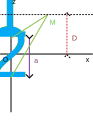
\includegraphics[scale=0.5]{schema6}

On suppose également l'écran loin des sources et M proche du centre.

On trouve que \(\delta = na(1-\frac{x^2+y^2}{2D^2})\) et \(\Delta \varphi  = \frac{2\pi}{\lambda_0}na(1-\frac{x^2+y^2}{2D^2})\). On en déduit \(I(M) = 2I_0(1+\cos(\frac{2\pi}{\lambda_0}na(1-\frac{x^2+y^2}{2D^2})))\)

La forme géométrique de l'interférogramme (lieux d'égale intensité). On cherche donc \(\Delta \varphi = Cst \iff x^2+y^2 = Cst\) qui est l'équation d'un cercle centré au centre de l'écran.

\subsection{Dispositifs interférentiels à division du front d'onde}
Pour avoir 2 sources cohérentes de m\^eme pulsation \(\omega\), on va partager le front d'onde d'une source en 2 pour en fabriquer 2 nouvelles, qui seront cohérentes.
\subsubsection{Trous de Young}
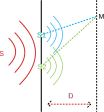
\includegraphics[scale=0.5]{young1}

On perce 2 petits trous dans un écran\marginWarning{Elle permet aussi de mettre en évidence que des éléments sont des ondes}.

On utilise alors un écran // à l'axe des sources et on peut se ramener aux calculs précédents.

\subsubsection{Biprisme de Fresnel}
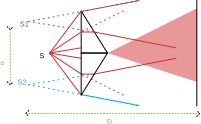
\includegraphics[scale=0.5]{biprisme}

Dans la zone d'interférence (ou champ d'interférence) tous les points sont illuminés par les sources virtuelles \(S_1,S_2\) et on se ramène au calcul précédent. %TODO trouver l'expression de la distance a

\subsection{Division d'amplitude}
\subsubsection{lame semie-réfléchissante}
Sur un dioptre plan, le rayon incident donne une onde réfléchie et un rayon réfractée (onde transmise). Les 2 ondes de sortie ont donc la m\^eme fréquence.

L'amplitude de l'onde incidente est divisée entre l'onde réfléchie et l'onde transmise.

On introduit les coefficients de réflexion \(r\) et de transmission \(t\)  par l'amplitude\marginInfo{On peut faire de m\^eme pour l'intensité} : \(\fo_r = \fo_i r, \fo_t = \fo_i t\).

\warningInfo{Nombre complexe}{Ces coefficients peuvent \^etre complexes, i.e. avoir une phase}

Par exemple, pour un dioptre plan en incidence normale, on a \[r = \frac{n_1-n_2}{n_1+n_2}, t = \frac{2n_1}{n_1+n_2}\]

Exemple 2 : Lame 50/50 : \(|r|=|t|\). Elle permet l'interférence de 2 ondes de m\^eme amplitude.

\subsection{lame à face parallèle}
On prend des lames de faces parallèles d'épaississeur e, d'indice n placées dans l'air.

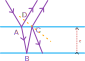
\includegraphics[scale=0.5]{lame}

Les 2 rayons correspondent à des OPPM et se croisent à l'infini (interférences observables au foyer d'une lentille).

On cherche la différence de marche entre ces deux ondes de m\^eme vecteur d'onde. Elle correspond à la différence de parcourt entre le point de départ A et les points d'arrivée C et D.

Donc \(\delta = (AB)+(BC)-(AD) = n(AB+BC) - AD = 2ne \cos(\theta_2)\)

\subsubsection{Interféromètre de Michelson}

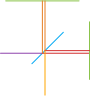
\includegraphics[scale=0.5]{michelson}

Le miroir de Michelson est un interféromètre optique qui permet de visualiser et de mesurer les \textbf{interférences d'ondes}. Le dispositif se compose des éléments suivants :

\begin{enumerate}
    \item Une \textbf{source lumineuse} (violet) monochromatique et cohérente (par exemple, un laser).
    \item Une \textbf{lame semi-réfléchissante} (bleu) (séparatrice de faisceau) qui divise le faisceau incident en deux.
    \item Deux \textbf{miroirs} (vert) (M1 et M2) placés aux extrémités des deux bras de l'interféromètre.
    \item Un \textbf{détecteur} ou un écran pour observer les franges d'interférence.
\end{enumerate}

Le faisceau incident est divisé en deux parties par la lame semi-réfléchissante. Chaque faisceau parcourt un bras de l'interféromètre (de longueurs respectives $L_1$ et $L_2$), est réfléchi par un miroir et retourne vers la lame. Les deux faisceaux se recombinent sur la lame, et le faisceau résultant, porteur de l'information d'interférence, est dirigé vers le détecteur.

L'observation de franges d'interférence est due à la \textbf{différence de marche optique} $\delta$ entre les deux faisceaux. Puisque chaque faisceau effectue un aller-retour dans son bras respectif, la différence de marche est donnée par :
\[ \delta = 2L_2 - 2L_1 = 2(L_2 - L_1) \]
On peut donc calculer la distance d :

\includegraphics[scale=0.5]{michel2}



 \end{document}
